\documentclass[14pt]{beamer}
\usefonttheme[onlymath]{serif}
\usepackage[normalem]{ulem}
\usepackage[T2A]{fontenc}
\usepackage[utf8]{inputenc}
\usepackage[english,russian]{babel}
\usepackage{amssymb,amsfonts,amsmath,mathtext}
\usepackage{cite,enumerate,float,indentfirst}
\usepackage{bm}

\graphicspath{{images/}}

\usetheme{Pittsburgh}
\usecolortheme{whale}

\setbeamercolor{footline}{fg=blue}
\setbeamertemplate{footline}{
  \leavevmode%
  \hbox{%
  \begin{beamercolorbox}[wd=.333333\paperwidth,ht=2.25ex,dp=1ex,center]{}%
    Павлович В. В. | selatnick@gmail.com
  \end{beamercolorbox}%
  \begin{beamercolorbox}[wd=.333333\paperwidth,ht=2.25ex,dp=1ex,center]{}%
    Минск, 2017
  \end{beamercolorbox}%
  \begin{beamercolorbox}[wd=.333333\paperwidth,ht=2.25ex,dp=1ex,right]{}%
  Стр. \insertframenumber{} из \inserttotalframenumber \hspace*{2ex}
  \end{beamercolorbox}}%
  \vskip0pt%
}

\newcommand{\itemi}{\item[\checkmark]}

\title{Поверхности Кунса}
\author{\small{%
\emph{Выступающий:}~Павлович Владислав}
\vspace{20pt}%
}
\date{\small{Минск, 2017}}

\begin{document}
\maketitle

\begin{frame}
\frametitle{Условие совместимости}
\center{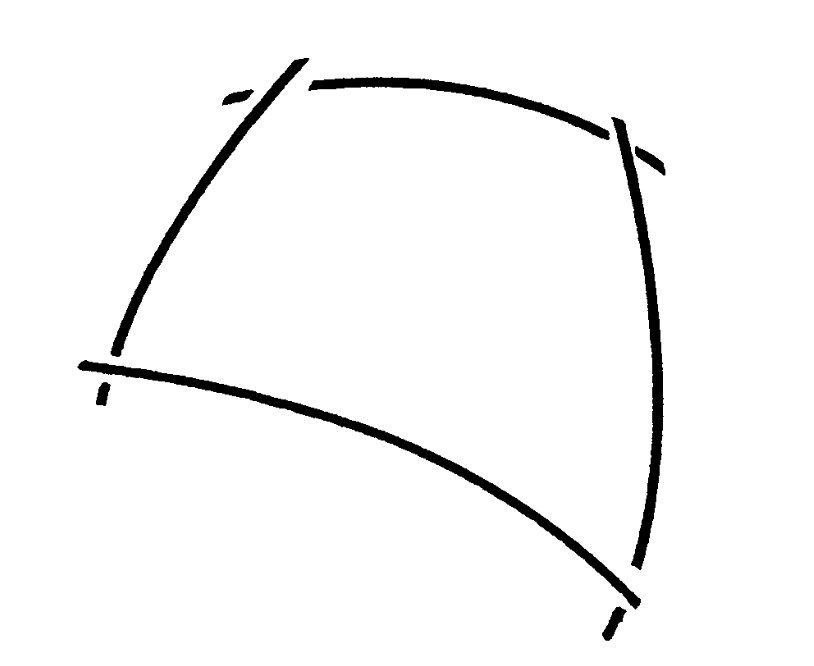
\includegraphics[width=0.9\linewidth]{incompatible_patch.png}}
\end{frame}

\begin{frame}
\frametitle{Условие совместимости}
\center{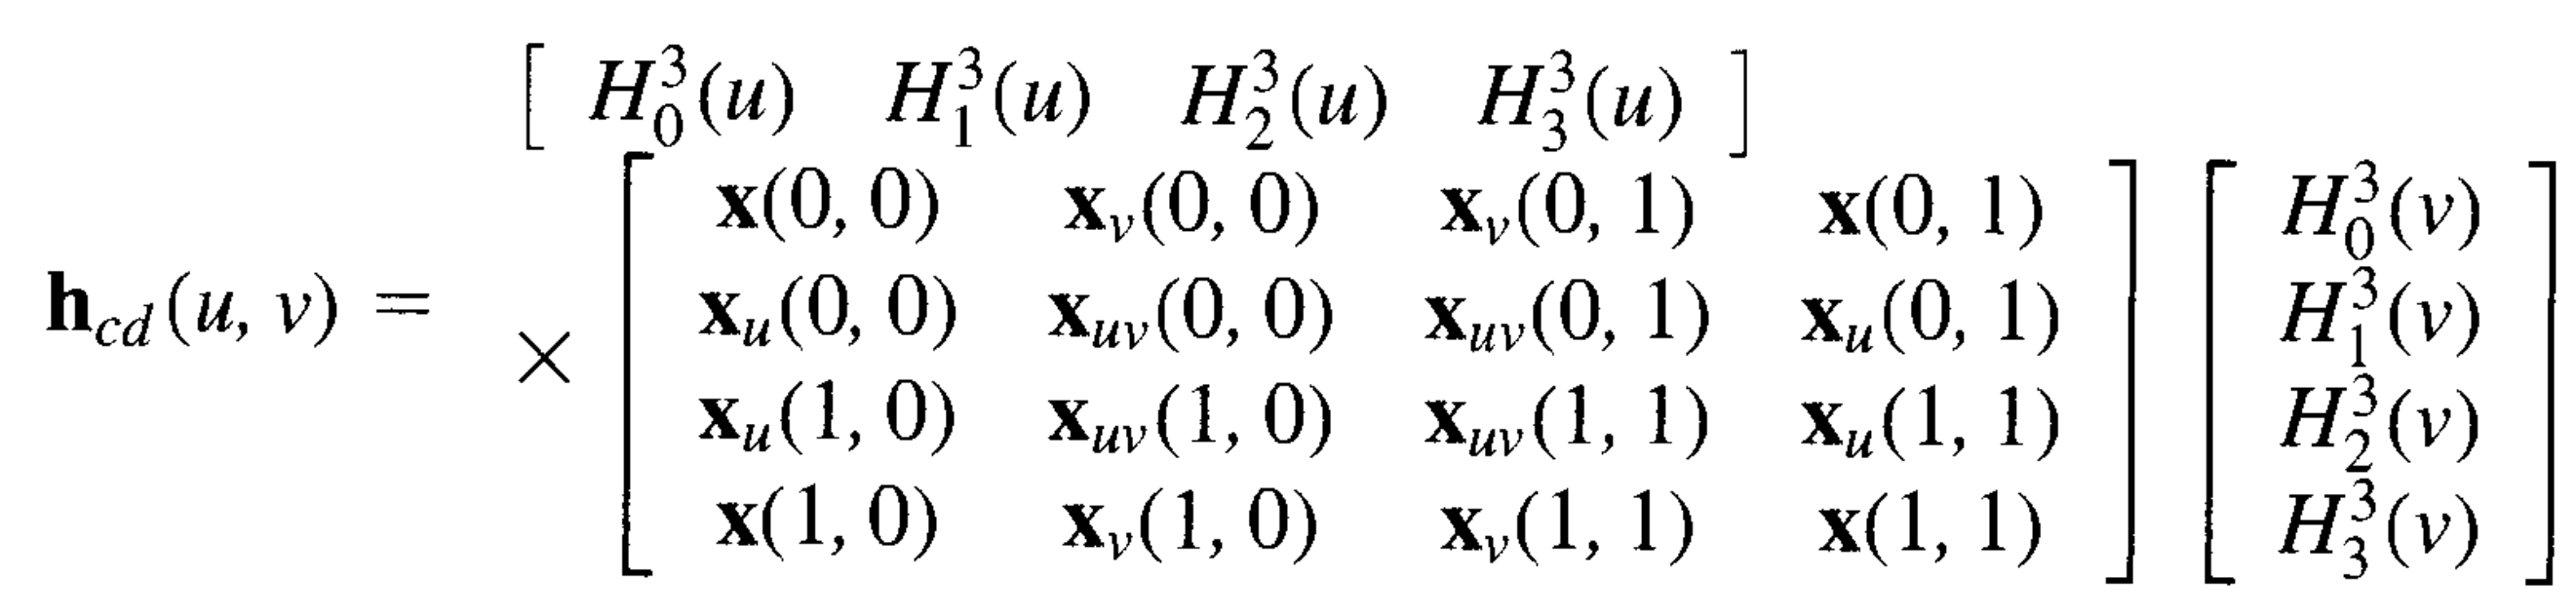
\includegraphics[width=1.0\linewidth]{twist_terms.png}}
\end{frame}

\begin{frame}
\frametitle{Условие совместимости}
Коэффициенты изгиба не обязяательно равны.
\center{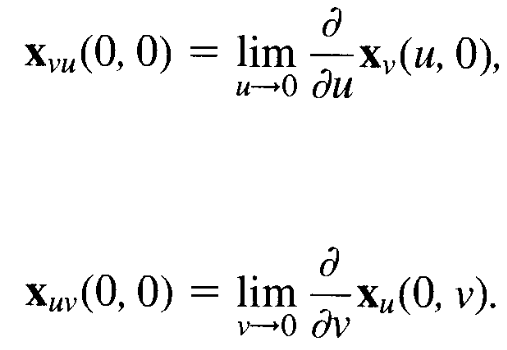
\includegraphics[width=0.5\linewidth]{x2.png}}
\end{frame}

\begin{frame}
\frametitle{Условие совместимости}
\center{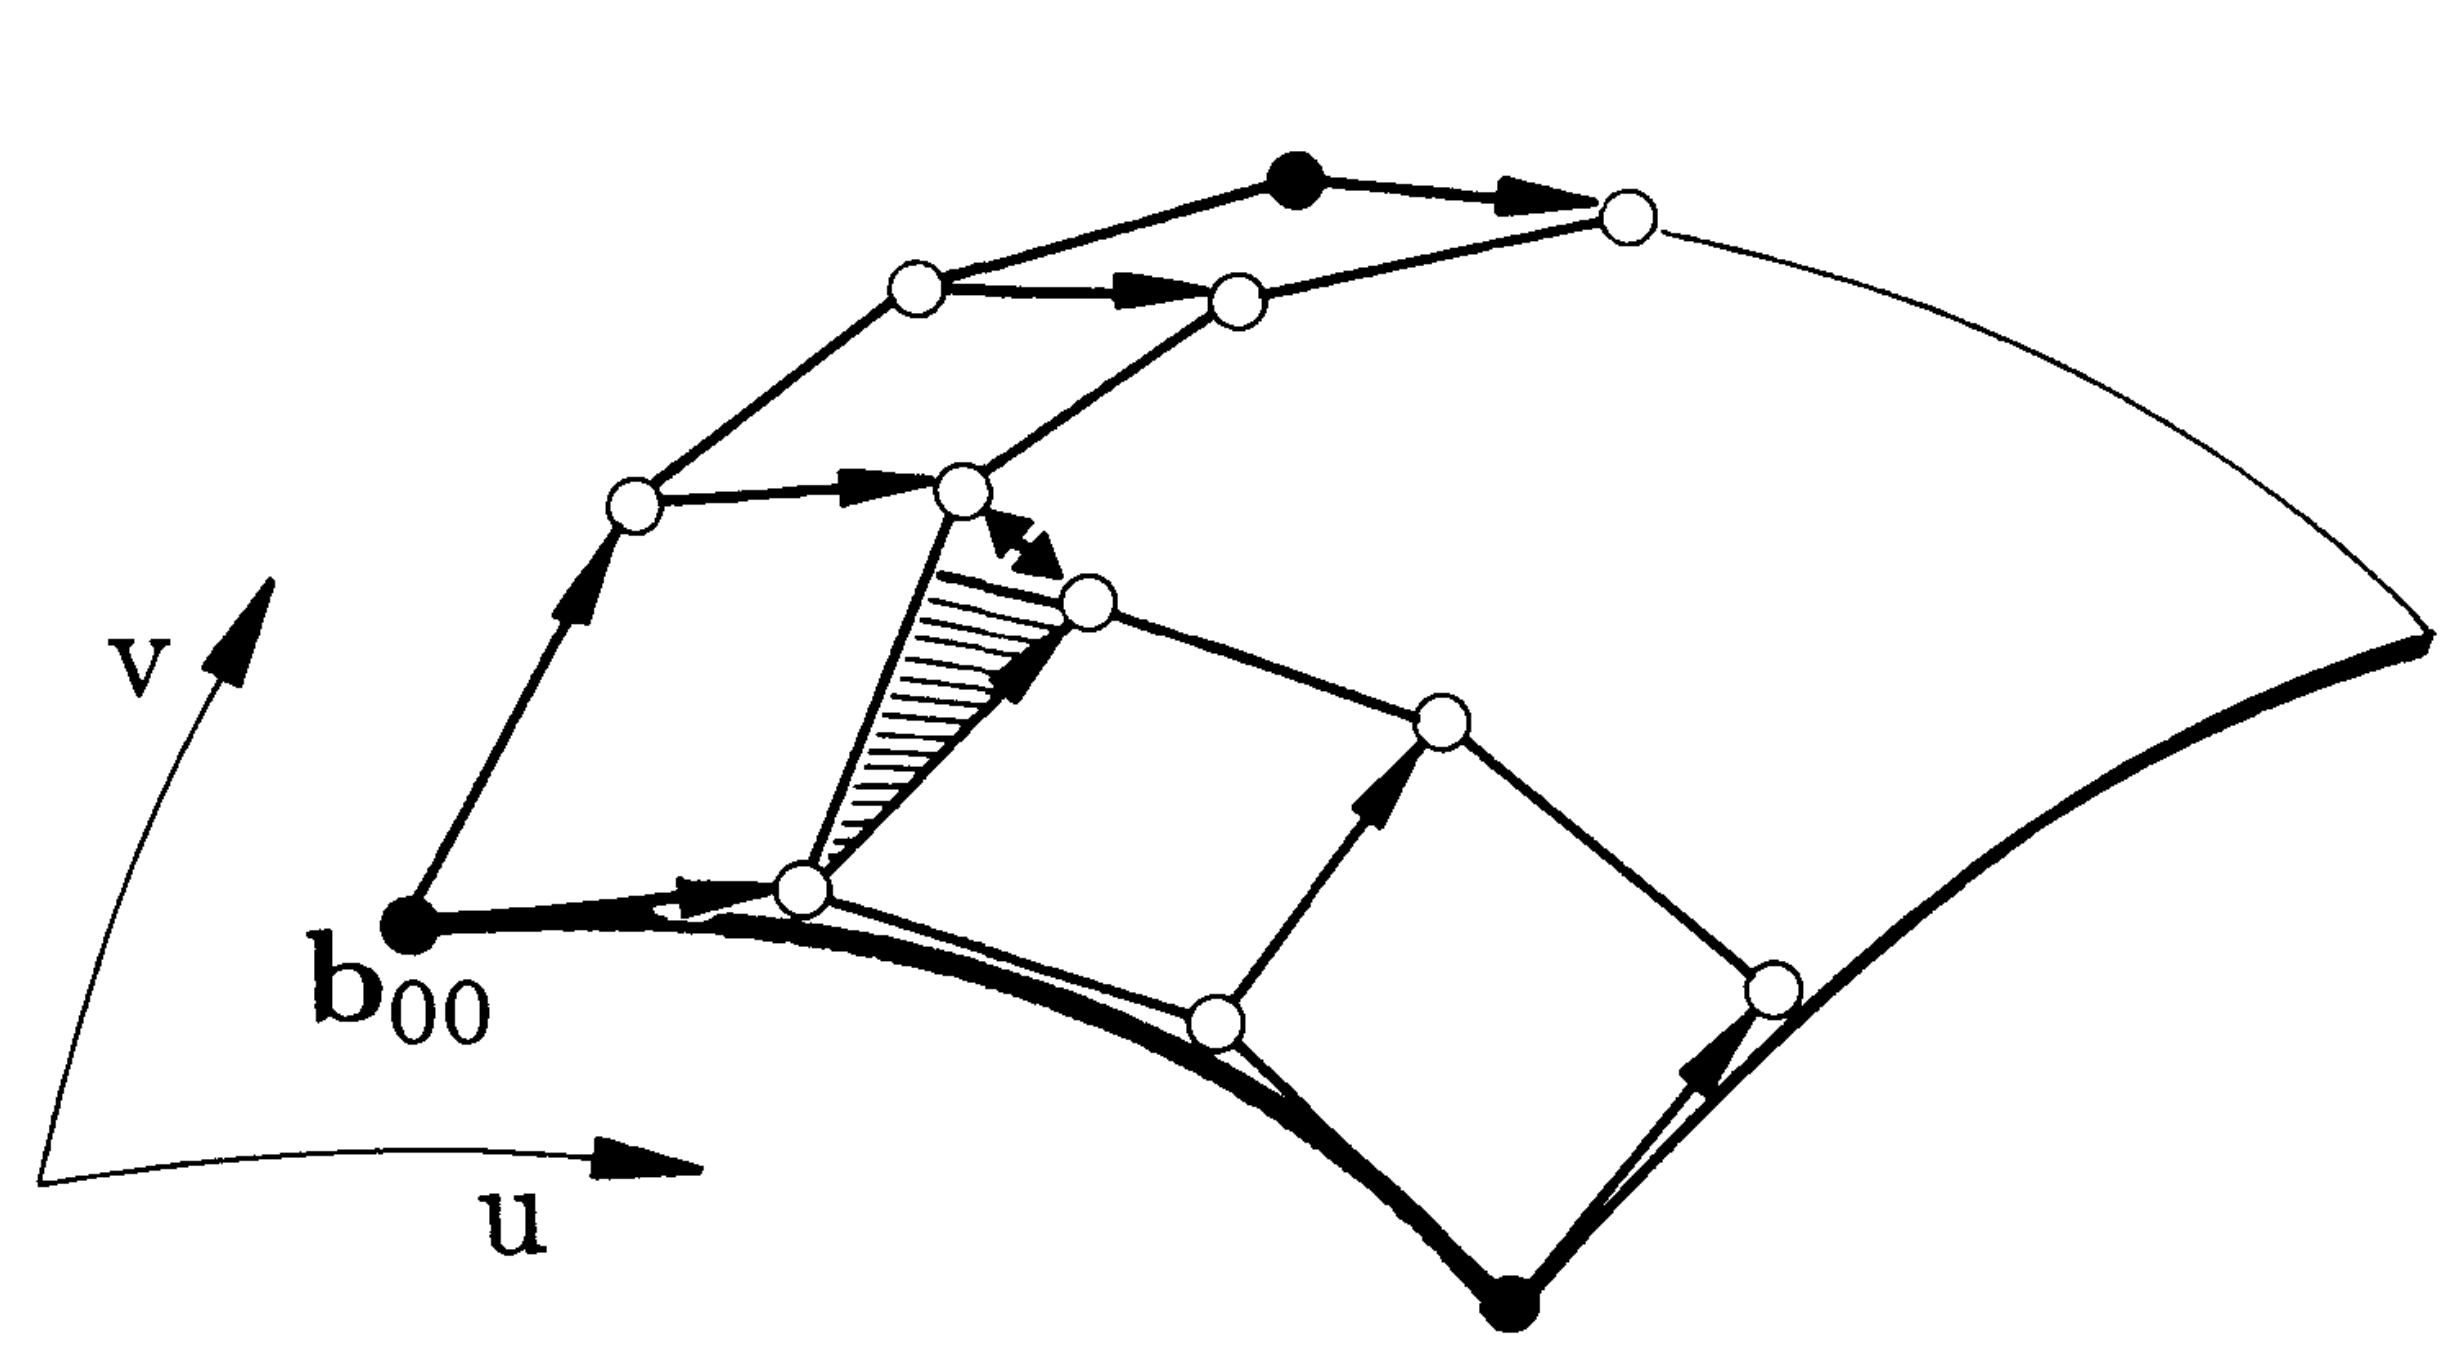
\includegraphics[width=1\linewidth]{different_twists.png}}
\end{frame}

\begin{frame}
\frametitle{Условие совместимости}
\begin{itemize}
  \item Выбрав одно из значений получаем частичную интерполяцию.
  \item Получится ещё хуже, если подставим нули вместе всех коэффициентов изгиба.
\end{itemize}
\end{frame}

\begin{frame}
\frametitle{Условие совместимости}
Методы решения:
\begin{itemize}
  \item Корректировка исходных кривых и избавление от несовместимостей.
  \item Квадрат Грегори: замена постоянных коэффициентов изгиба на переменные.
\end{itemize}
\end{frame}

\begin{frame}
\frametitle{Условие совместимости. Квадрат Грегори}
\center{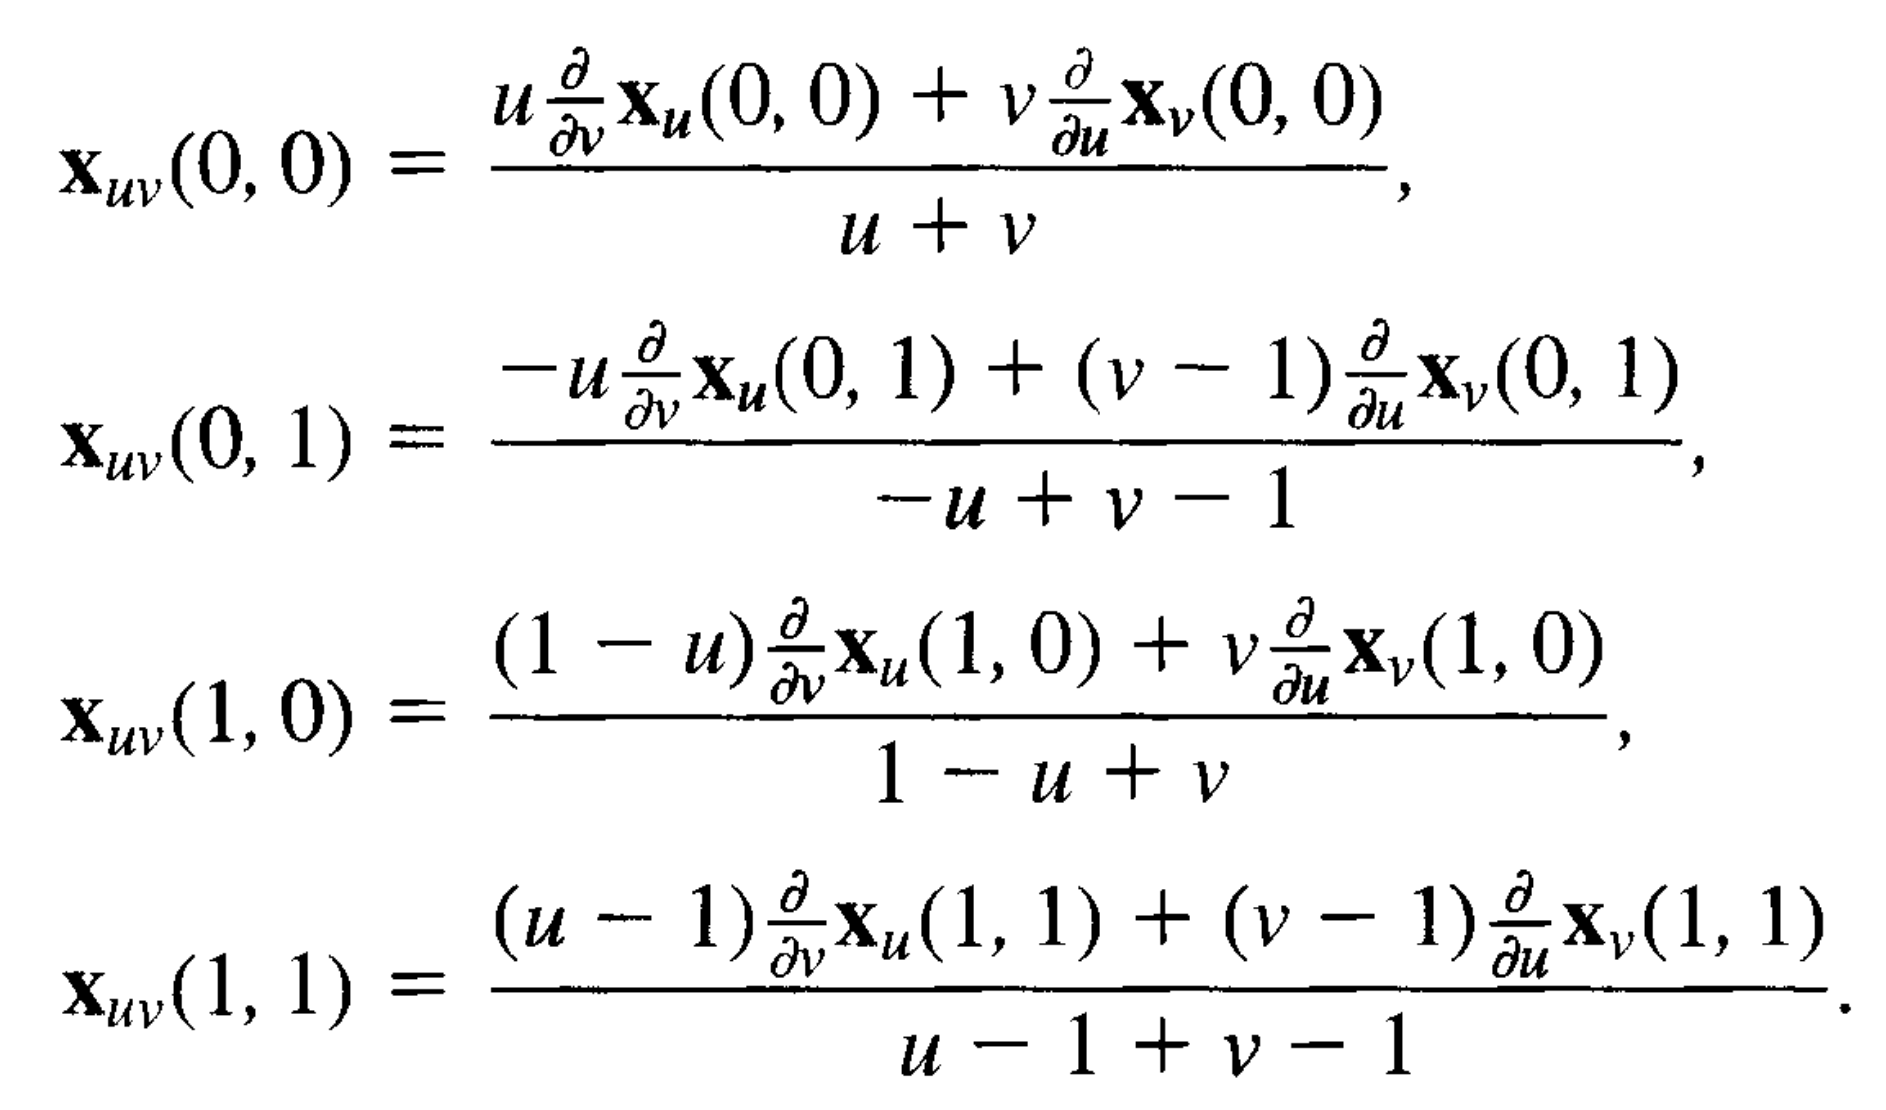
\includegraphics[width=0.95\linewidth]{gregory.png}}
\end{frame}

\begin{frame}
\frametitle{Условие совместимости}
Методы решения:
\begin{itemize}
  \item Изгиб не является непрерывным.
  \item Разные значения в зависимости от того, с какой стороны подходить к углу.
\end{itemize}
\end{frame}

\begin{frame}
\frametitle{Контрольные сети}
Дано:
\begin{itemize}
  \item 4 граничные кривые (B-сплайн или кривая Безье).
  \item Противоположные кривые имеют одинаковую степеньи определены одной и той
  же последовательностью узловых точек.
\end{itemize}
Задача:
\begin{itemize}
  \item Найти контрольную сеть, которая распологается между граничными кривыми,.
\end{itemize}
\end{frame}

\begin{frame}
\frametitle{Контрольные сети}
\center{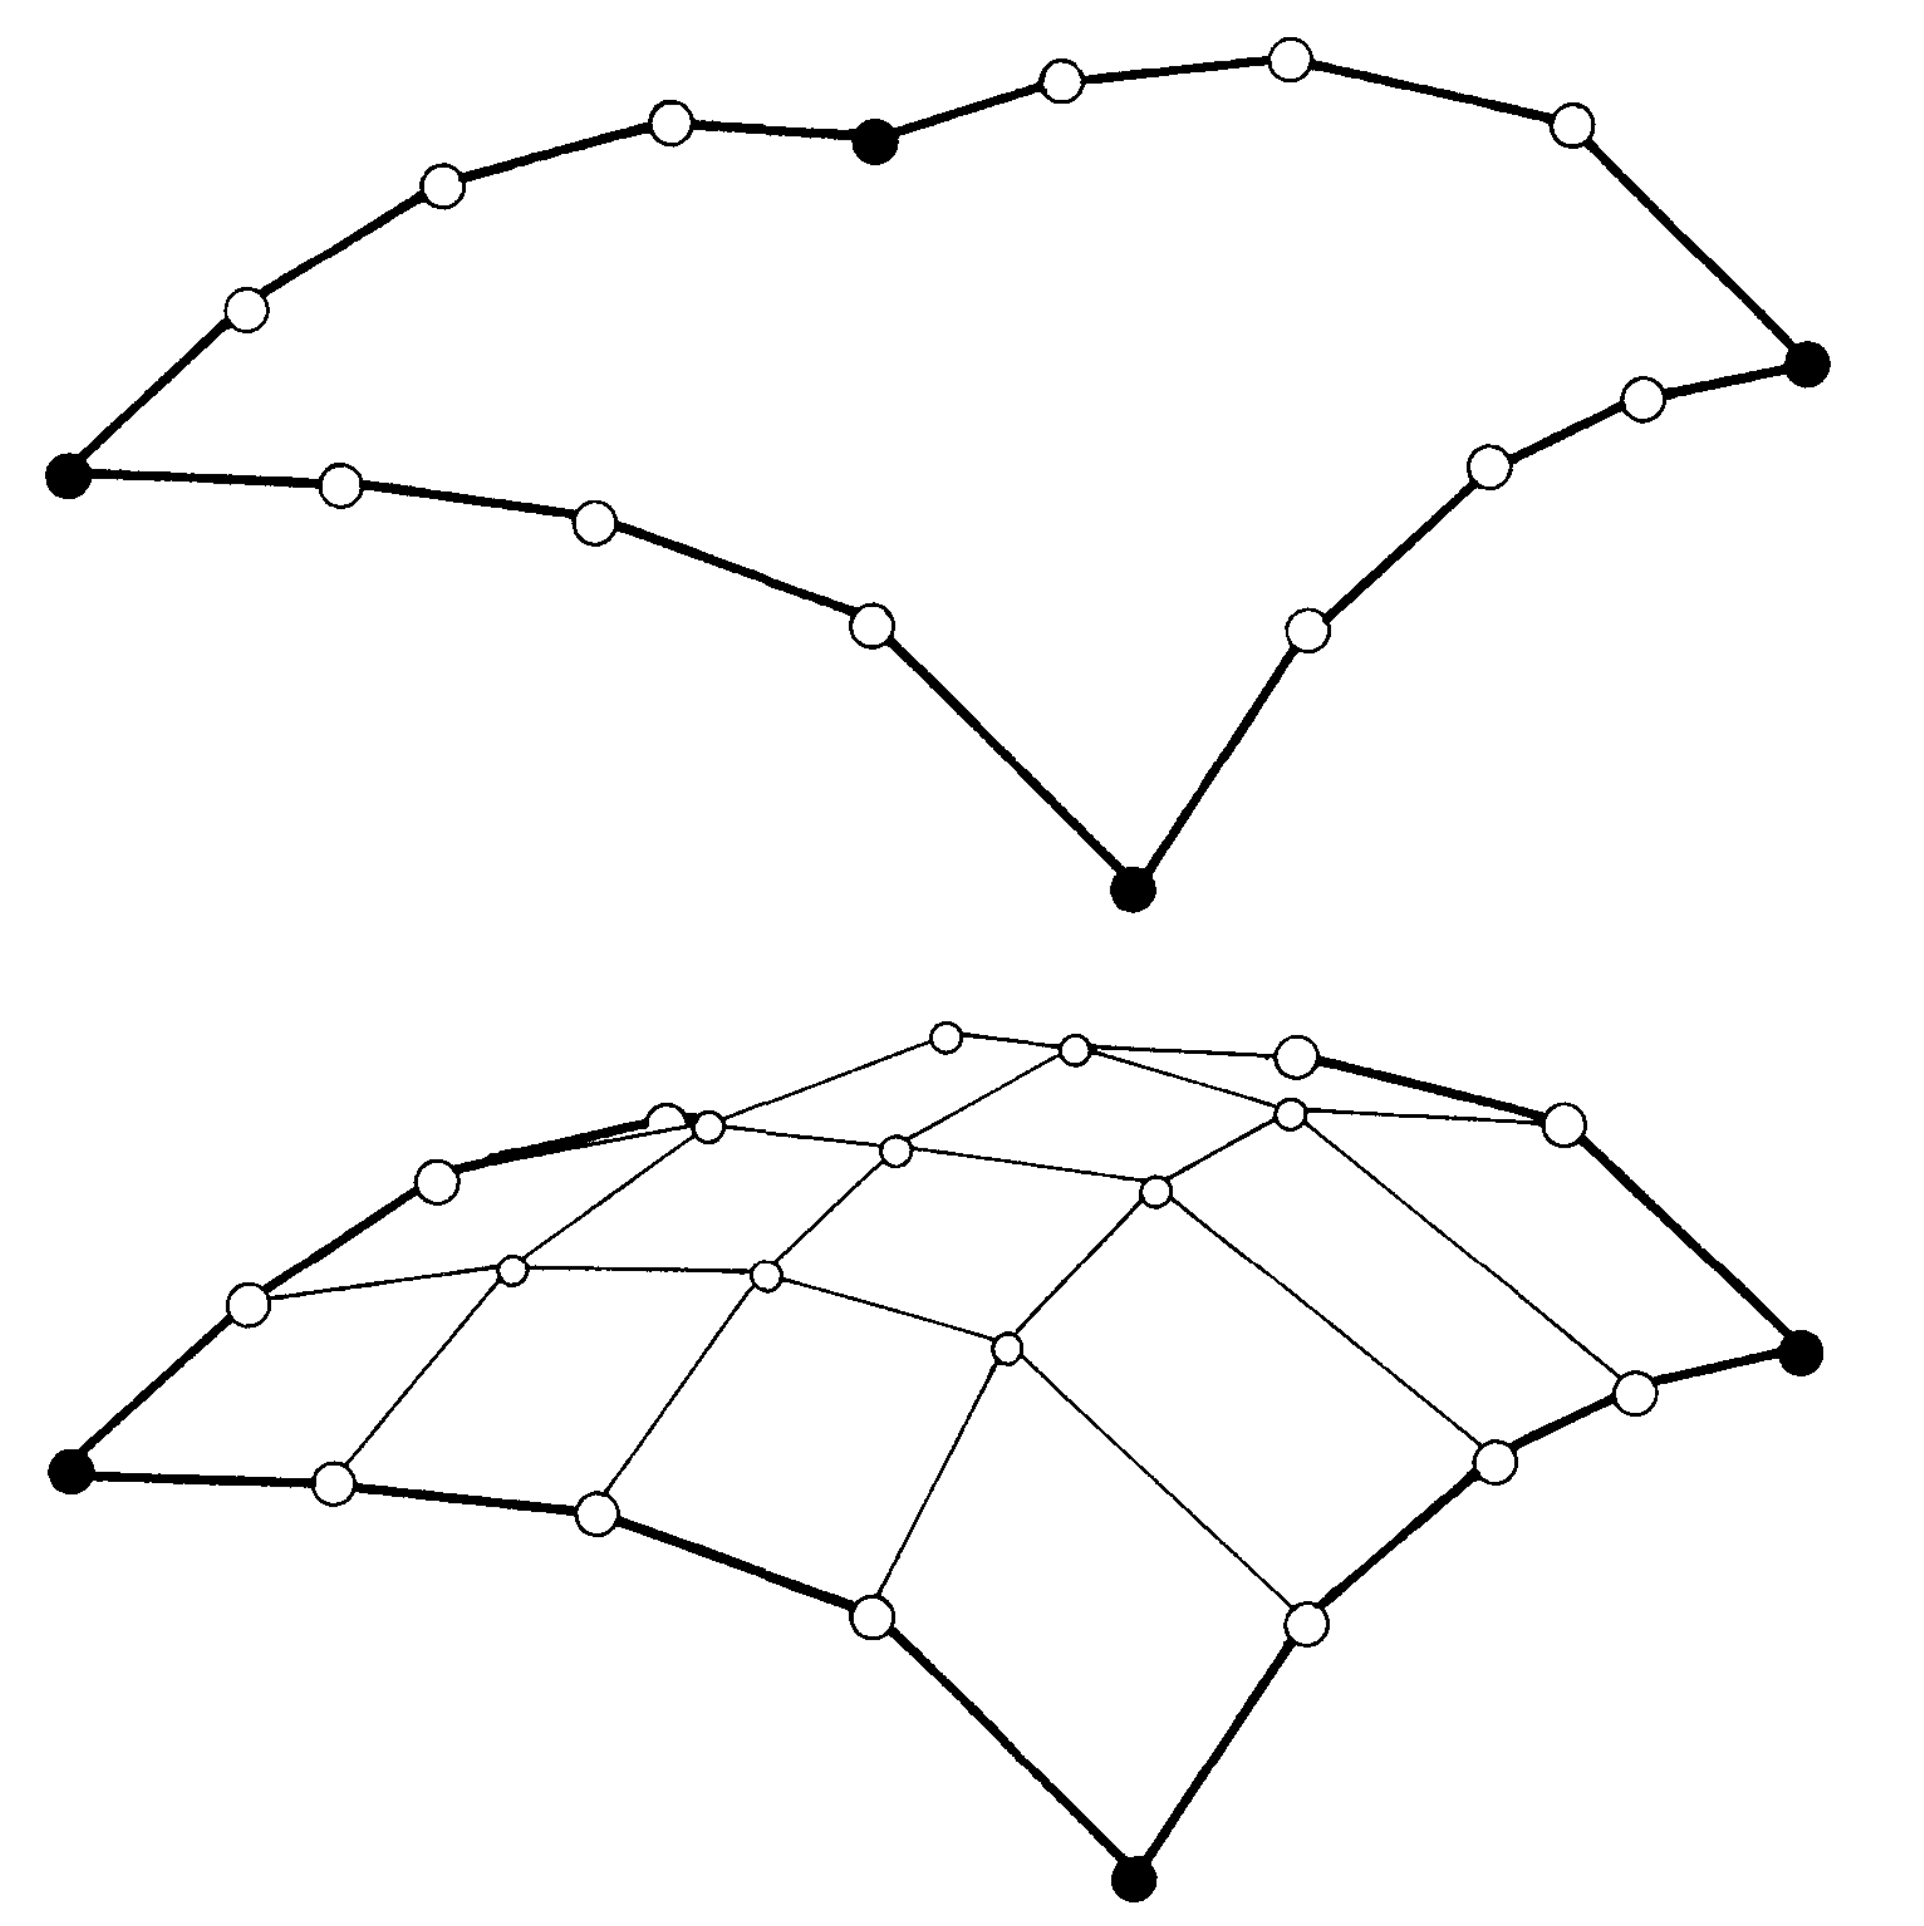
\includegraphics[width=0.6\linewidth]{control_net.png}}
\end{frame}

\begin{frame}
\frametitle{Контрольные сети}
\begin{itemize}
  \item Интерпретируем границы как кусочно-линейные кривые.
  \item Вычисляем билинейно смешанную поверхность Кунса, которая их интерполирует.
  \item Полученная поверхность будет кусочно-билинейной.
\end{itemize}
\end{frame}

\begin{frame}
\frametitle{Трансляционные поверхности}
$c_1(u), c_2(u)$ - кривые с общей точкой пересечения $a$.
\begin{align*}
  &t(u, v) = c_1(u) + c_2(v) - a\\
  &\dfrac{\partial^2}{\partial u \partial v}t(u, v) = 0
\end{align*}
\end{frame}

\begin{frame}
\frametitle{Трансляционные поверхности}
\center{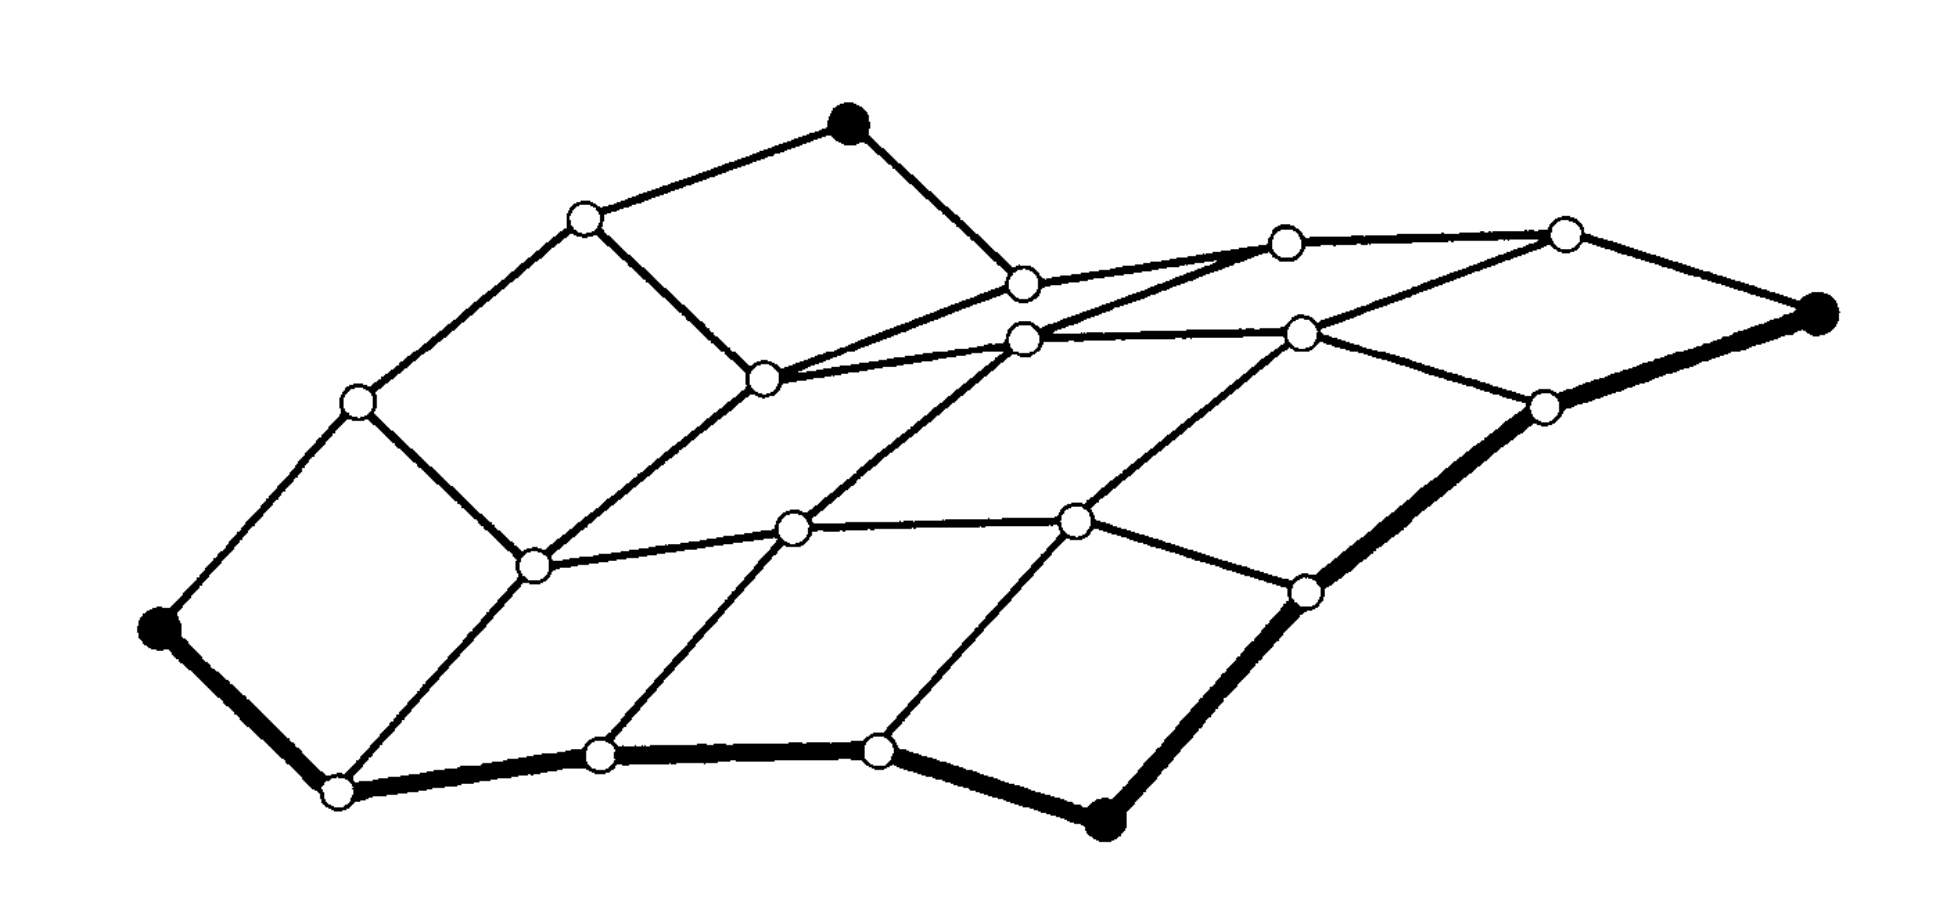
\includegraphics[width=1\linewidth]{translation_example.png}}
\end{frame}

\begin{frame}
\frametitle{Трансляционные поверхности}
\textbf{Выпуклая комбинация} - взвешенная сумма четырёх поверхностей.
\center{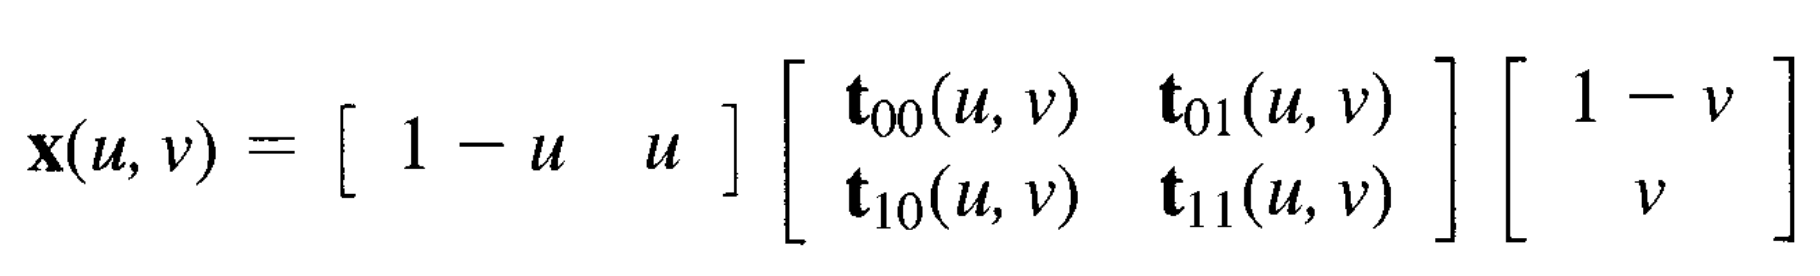
\includegraphics[width=1\linewidth]{translation_coons.png}}
\end{frame}

\begin{frame}
\frametitle{Поверхности Гордона}
\center{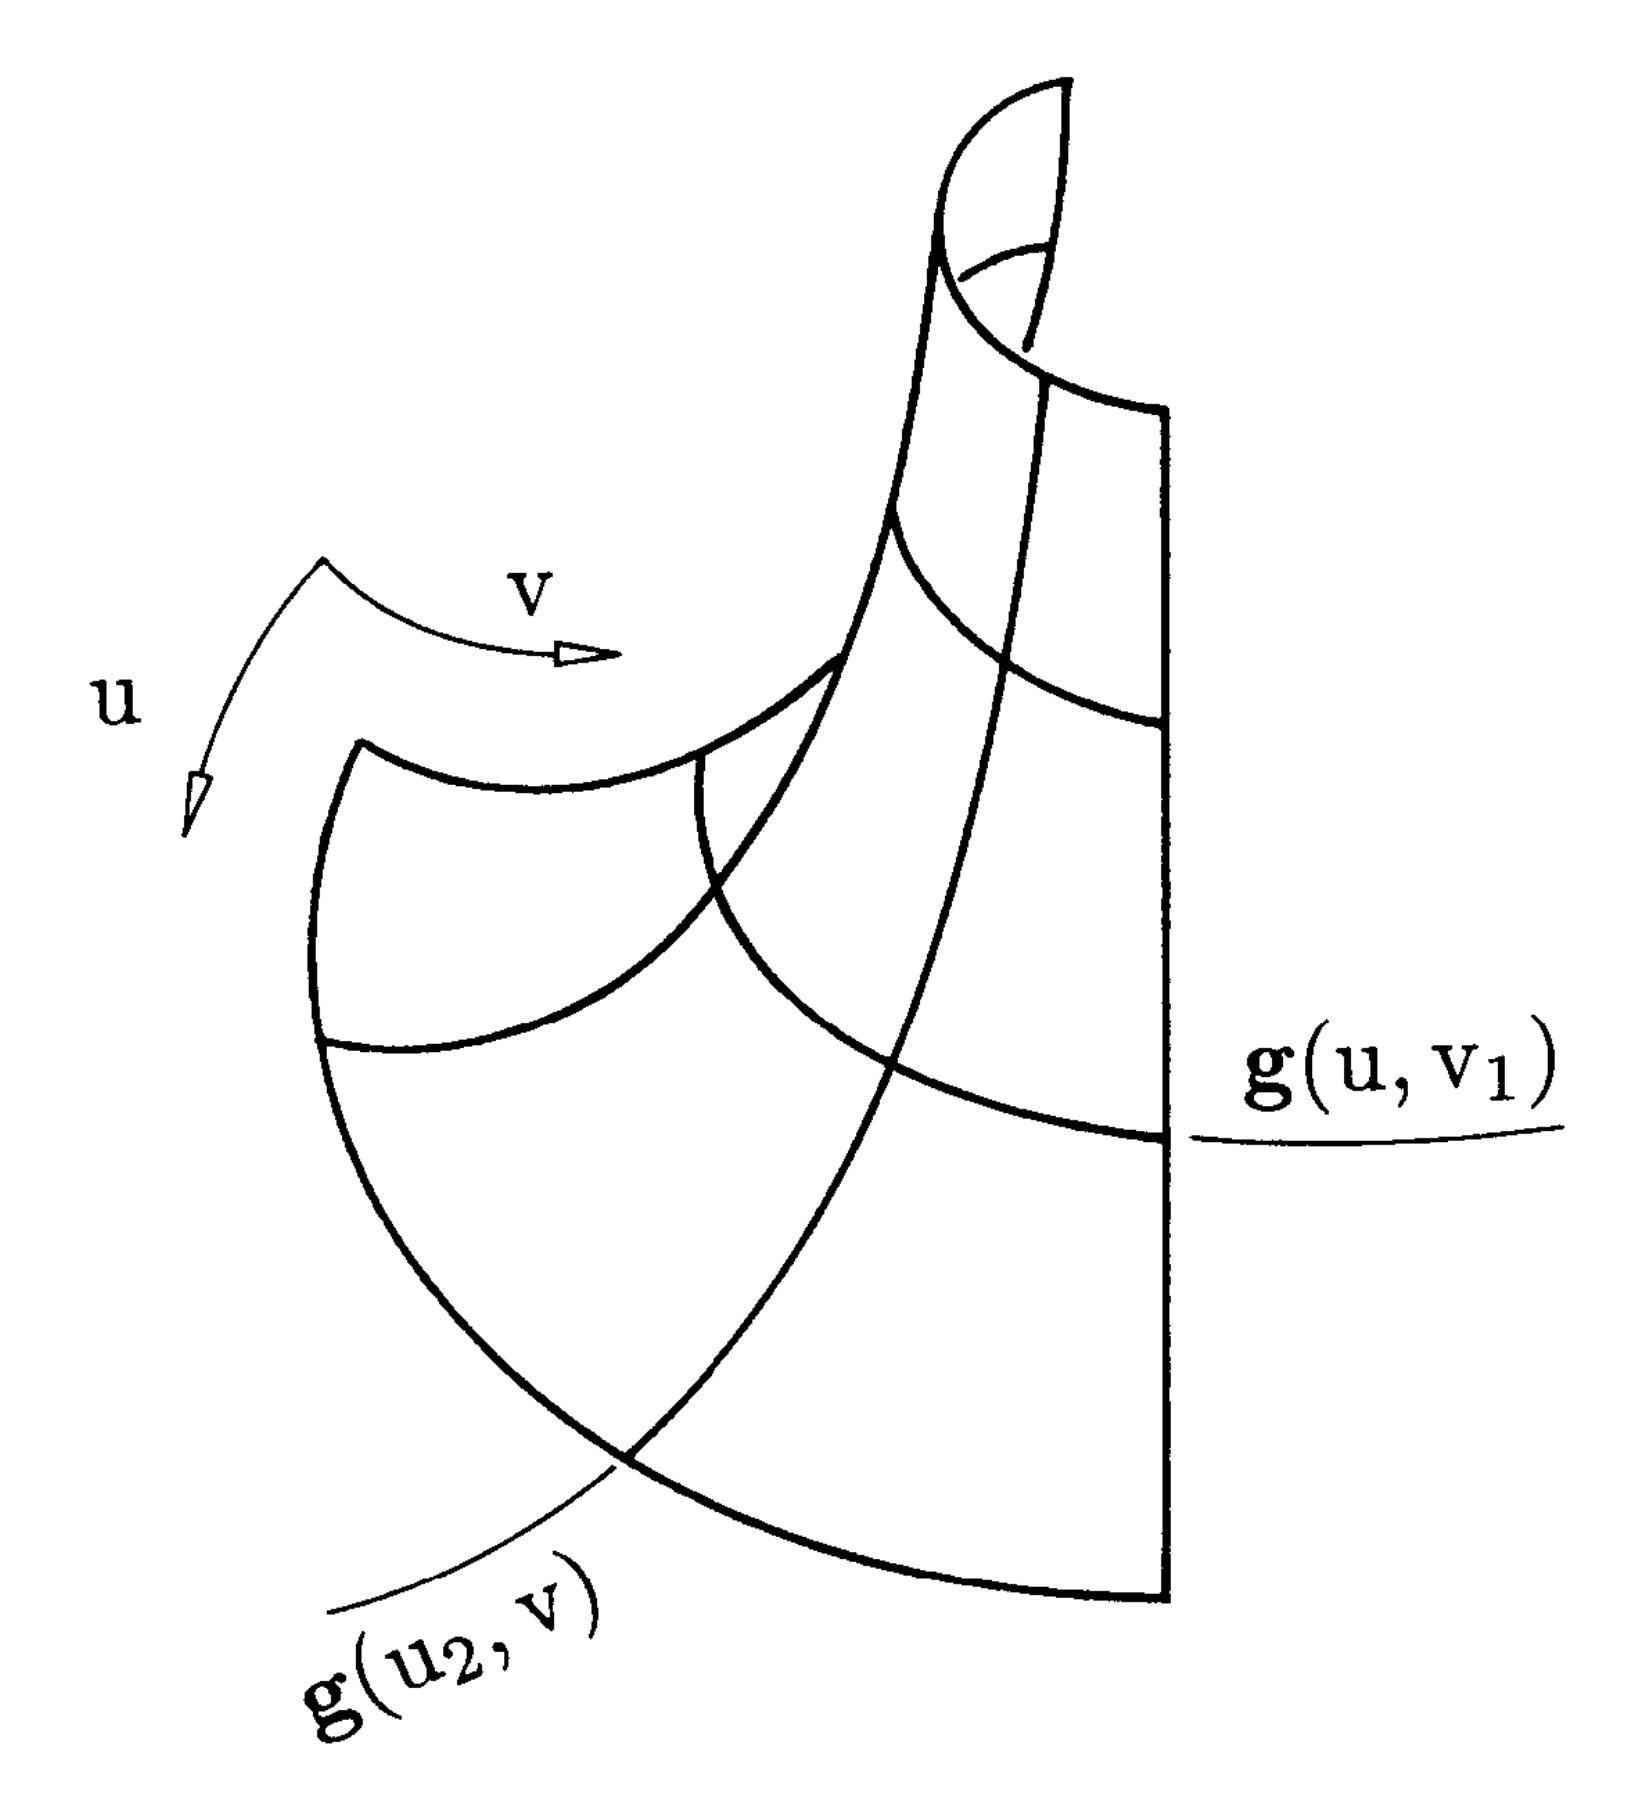
\includegraphics[width=0.6\linewidth]{gordon.png}}
\end{frame}

\begin{frame}
\frametitle{Поверхности Гордона}
\center{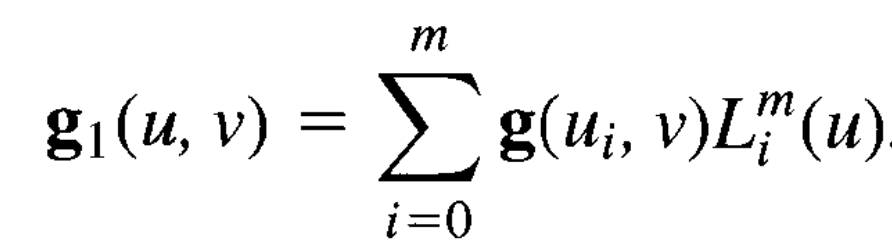
\includegraphics[width=0.6\linewidth]{gordon_block1.png}}
\center{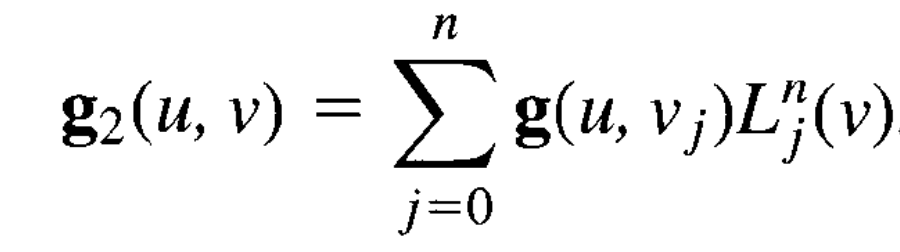
\includegraphics[width=0.6\linewidth]{gordon_block2.png}}
\center{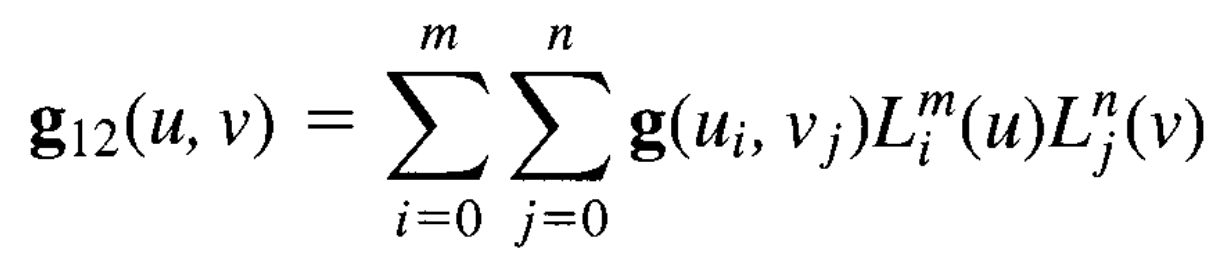
\includegraphics[width=0.6\linewidth]{gordon_block12.png}}
\center{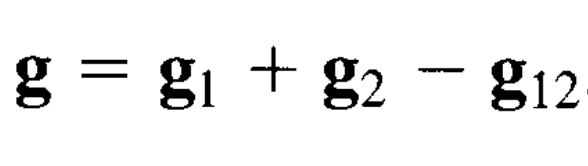
\includegraphics[width=0.6\linewidth]{gordon_sum.png}}
\end{frame}

\begin{frame}
\frametitle{Булевы суммы}
\center{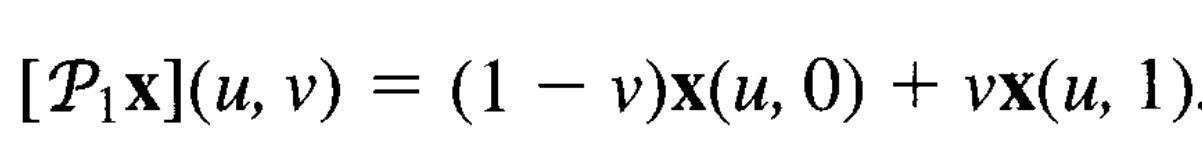
\includegraphics[width=0.6\linewidth]{boolean_op1.png}}
\center{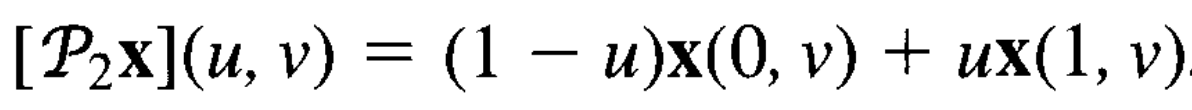
\includegraphics[width=0.6\linewidth]{boolean_op2.png}}
\center{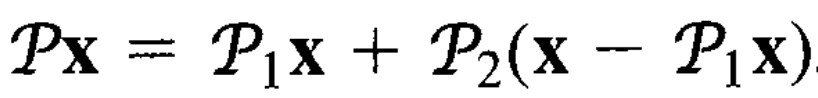
\includegraphics[width=0.4\linewidth]{boolean_sum.png}}
\center{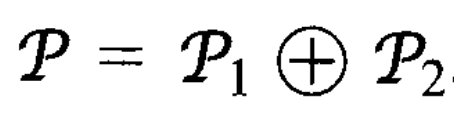
\includegraphics[width=0.3\linewidth]{boolean_short.png}}
\end{frame}

\begin{frame}
\frametitle{Треугольные поверхности Кунса}
\center{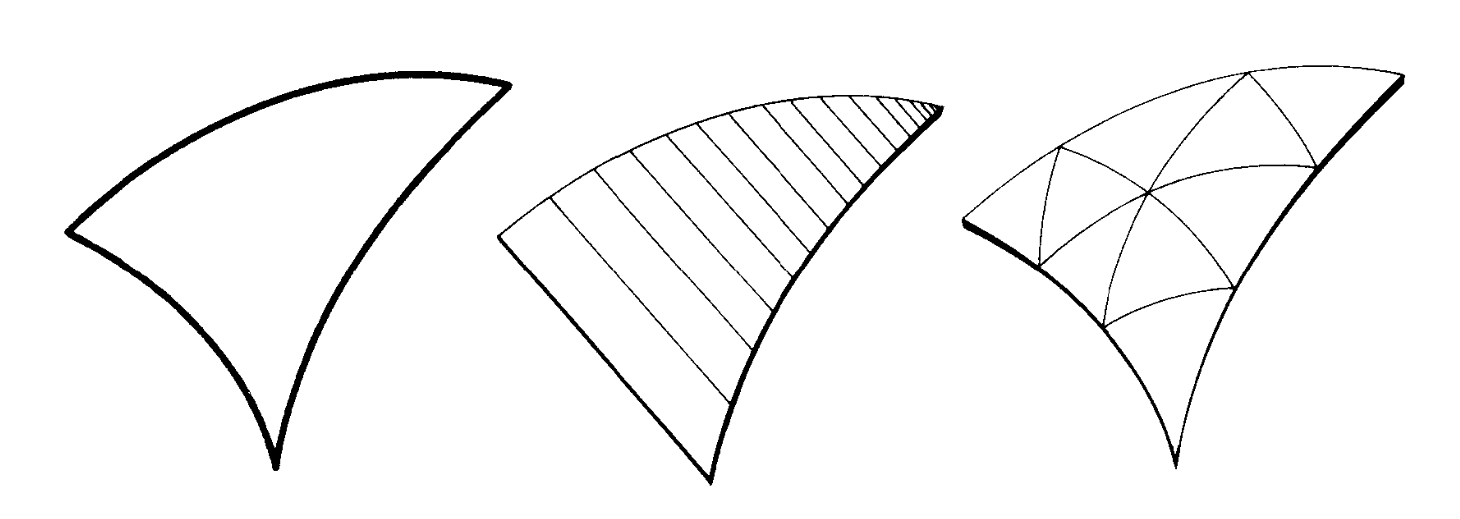
\includegraphics[width=1\linewidth]{triangular_patch.png}}
\end{frame}

\begin{frame}
\frametitle{Треугольные поверхности Кунса}
\begin{align*}
  &\bm{x}(0, v, w), \bm{x}(u, 0, w), \bm{x}(u, v, 0)\\
  &P_1\bm{x(u)} = (1 - r)\bm{x}(u, 0, w) + r\bm{x}(u, v, 0), r = \dfrac{v}{v + w}\\
  &P_2\bm{x(u)} = (1 - s)\bm{x}(u, v, 0) + s\bm{x}(0, v, w), s = \dfrac{w}{v + w}\\
  &P_3\bm{x(u)} = (1 - t)\bm{x}(u, 0, w) + t\bm{x}(0, v, w), t = \dfrac{v}{v + u}\\
\end{align*}
Рациональны по $u, v, w$ и линейны по $r, s, t$.
\end{frame}

\begin{frame}
\frametitle{Треугольные поверхности Кунса}
Возможные комбинации:

\begin{itemize}
  \item $P = P_1 \oplus P_2$.
  \item $P = uP_1x + vP_2x + wP_3x$.
\end{itemize}
\end{frame}

\begin{frame}
\frametitle{Треугольные поверхности Кунса}
\begin{align*}
  &\bm{x}(0, v, w), \bm{x}(u, 0, w), \bm{x}(u, v, 0)\\
  &P_1\bm{x(u)} = H_0^3(r)\bm{x}(u, 0, w) + H_1^3(r)\bm{x}_1(u, 0, w)\\
    &+ H_2^3(r)\bm{x}_1(u, v, 0) + H_3^3(r)\bm{x}(u, v, 0)\\
  &P_1\bm{x(u)} = H_0^3(r)\bm{x}(u, v, 0) + H_1^3(r)\bm{x}_2(u, v, 0)\\
    &+ H_2^3(r)\bm{x}_1(0, v, w) + H_3^3(r)\bm{x}(0, v, w)\\
  &P_1\bm{x(u)} = H_0^3(r)\bm{x}(u, 0, w) + H_1^3(r)\bm{x}_1(u, 0, w)\\
    &+ H_2^3(r)\bm{x}_1(u, 0, w) + H_3^3(r)\bm{x}(0, v, w)\\
\end{align*}
\end{frame}


\begin{frame}
\frametitle{Треугольные поверхности Кунса}
\begin{align*}
  &x_1(u) = (v + w)D_{e2 - e3}x(u)\\
  &x_2(u) = (u + w)D_{e3 - e1}x(u)\\
  &x_2(u) = (u + v)D_{e2 - e1}x(u)\\
\end{align*}
\end{frame}

\begin{frame}
\frametitle{Треугольные поверхности Кунса}
\begin{align*}
  &P_1\bm{x(u)} = u\bm{x}(1, 0, 0) + (1 - u)\bm{x}(0, r, 1 - r); r = \dfrac{v}{v + w}\\
  &P_2\bm{x(u)} = v\bm{x}(0, 1, 0) + (1 - v)\bm{x}(1 - s, 0, s); s = \dfrac{u}{u + w}\\
  &P_3\bm{x(u)} = w\bm{x}(0, 0, 1) + (1 - w)\bm{x}(1 - t, t, 0); t = \dfrac{u}{u + v}\\
\end{align*}
\end{frame}

\begin{frame}
\frametitle{Треугольные поверхности Кунса}
\begin{align*}
  P &= P_1 \oplus P_2 \oplus P_3\\
    &= P_1 + P_2 + P_3 - P_1P_2 - P_2P_3 - P_1P_3 + P_1P_2P_3
\end{align*}
\end{frame}

\begin{frame}
\frametitle{Треугольные поверхности Кунса. Подход Нельсона}
\center{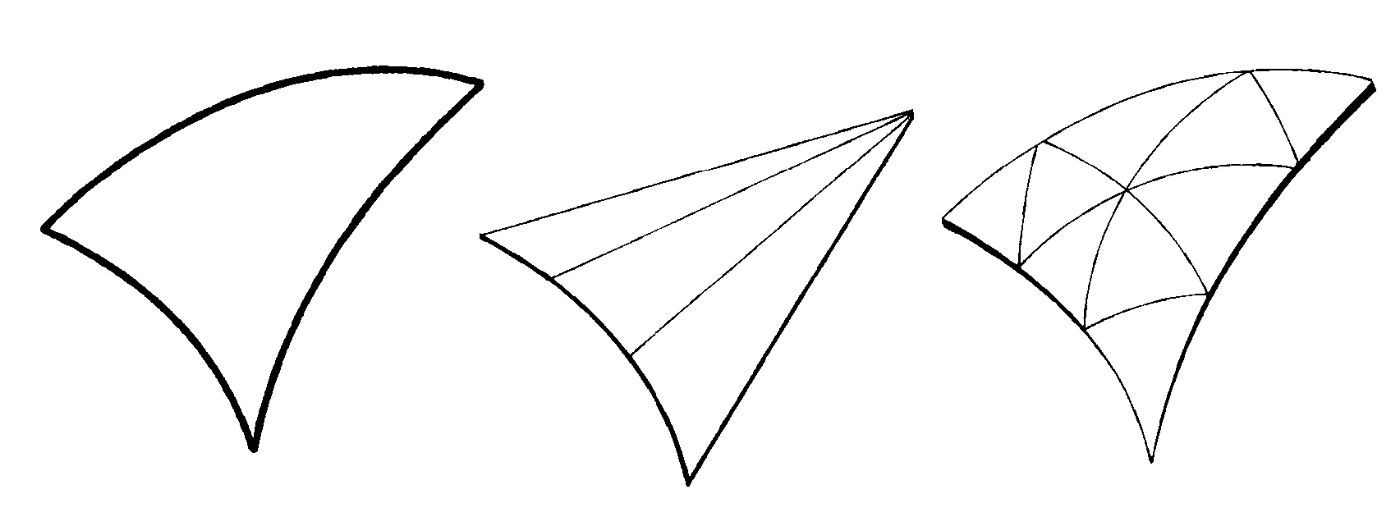
\includegraphics[width=1\linewidth]{nielson.png}}
\end{frame}

\end{document}
